\documentclass[a4paper, 12pt]{article}
\usepackage[top=1.8cm, bottom=1.8cm, left=1.5cm, right=1.5cm]{geometry}
\usepackage{float}
\usepackage[utf8]{inputenc}
\usepackage{pgfplots}
\pgfplotsset{width=10cm, compat=1.18}
\usepackage{multirow}



\begin{document}
	
	\begin{center}
		Universidade Federal do Rio Grande do Norte
		
		Departamento de Engenharia da Computação e Automação  
		
		DCA3703 - Programação Paralela  
		
		\textbf{Tarefa 17: Estruturas de Dados Não Contíguas em MPI}  
		
		\textbf{Aluno:} Daniel Bruno Trindade da Silva  
	\end{center}  
	
	\section{Introdução}
	
	\hspace{0.62cm}Este relatório tem como objetivo apresentar os conhecimentos adquiridos durante o desenvolvimento da Tarefa 17 da disciplina de Programação Paralela. A atividade teve como objetivo reimplementar o código da tarefa 16 distribuindo as colunas da matriz entre os processos, permitindo que cada um calculasse uma contribuição parcial para todos os elementos do vetor 'y'. ´Por fim, o relatório discute as diferenças de acesso à memória e desempenho desta abordagem em comparação com a distribuição por linhas.
	
	\section{Enunciado}
	
	\hspace{0.62cm}Reimplemente a tarefa 16, agora distribuindo as colunas entre os processos. Utilize \texttt{MPI\_Type\_vector} e \texttt{MPI\_Type\_create\_resized} para definir um tipo derivado que represente colunas da matriz. Use \texttt{MPI\_Scatter} com esse tipo para distribuir blocos de colunas, e \texttt{MPI\_Scatter} ou cópia manual para enviar os segmentos correspondentes de x. Cada processo deve calcular uma contribuição parcial para todos os elementos de y e usar \texttt{MPI\_Reduce} com \texttt{MPI\_SUM} para somar os vetores parciais no processo 0. Discuta as diferenças de acesso à memória e desempenho em relação à distribuição por linhas.
	
	\section{Desenvolvimento}
	\hspace{0.62cm}Fizemos a reimplementação do código original, alterando a estratégia de paralelização para realizar a distribuição da matriz por colunas entre os processos, utilizando tipos derivados do MPI. Essa abordagem visa uma distribuição mais eficiente da matriz e do vetor, aproveitando melhor os recursos de comunicação da biblioteca MPI.
	
	\subsection{Criação do Tipo Derivado para Representação das Colunas}
	\hspace{0.62cm}A matriz A é armazenada em memória de forma contígua linha a linha (ordem row-major). Como o objetivo é distribuir blocos de colunas entre os processos, foi necessário criar um tipo derivado que representasse de forma lógica esse agrupamento, apesar de sua não contiguidade na memória.
	
	Para isso, utilizamos inicialmente a função \texttt{MPI\_Type\_vector}. Esse construtor cria um tipo derivado com múltiplos blocos, permitindo a seleção de elementos com espaçamento regular:
	
	\begin{verbatim}
		MPI_Type_vector(M, cols_per_proc, N, MPI_UNSIGNED_CHAR, &column_type);
	\end{verbatim}
	
	Onde:
	\begin{itemize}
		\item \textbf{M}: número de blocos, correspondente ao número de linhas da matriz.
		
		\item \texttt{cols\_per\_proc}: número de elementos consecutivos a serem enviados por linha, isto é, a quantidade de colunas atribuídas a cada processo.
		
		\item \textbf{N}: espaçamento entre os inícios de blocos, igual ao número total de colunas da matriz.
		
		\item \texttt{MPI\_UNSIGNED\_CHAR}: tipo base, equivalente a \texttt{uint8\_t}.
	\end{itemize}
	
	Porém, o tipo criado por \texttt{MPI\_Type\_vector} possui um extent (extensão) maior do que o necessário para o envio contínuo entre processos. Por isso, utilizamos a função \texttt{MPI\_Type\_create\_resized} para ajustar esse tamanho, garantindo que o \texttt{MPI\_Scatter} realize a comunicação corretamente:
	
	\begin{verbatim}
		MPI_Type_create_resized(
		    column_type, 0, 
		    cols_per_proc * sizeof(uint8_t),
		    &resized_column_type
		);
		MPI_Type_commit(&resized_column_type);	
	\end{verbatim}
	
	\subsection{Distribuição dos Dados com MPI\_Scatter}
	\hspace{0.62cm}Com o tipo derivado criado, foi possível empregar \texttt{MPI\_Scatter} para distribuir diretamente os blocos de colunas da matriz entre os processos:
	
	\begin{verbatim}
		MPI_Scatter(
		    &A[0][0], 1,
		    resized_column_type,
		    local_A, M * cols_per_proc,
		    MPI_UNSIGNED_CHAR, 0,
		    MPI_COMM_WORLD
		);
	\end{verbatim}
	
	\begin{itemize}
		\item O processo raiz (rank 0) envia uma unidade do tipo derivado para cada processo.
		
		\item Cada processo recebe em \texttt{local\_A} seu bloco de colunas, já linearizado com tamanho M * \texttt{cols\_per\_proc}.
	\end{itemize}
	
	Já a distribuição do vetor x foi realizada em paralelo, utilizando um segundo \texttt{MPI\_Scatter}:
	
	\begin{verbatim}
		MPI_Scatter(
		    x, cols_per_proc,
		    MPI_UNSIGNED_CHAR,
		    local_x, cols_per_proc,
		    MPI_UNSIGNED_CHAR, 0,
		    MPI_COMM_WORLD
		);		
	\end{verbatim}
	
	\subsection{Cálculo da Contribuição Parcial e Redução com \texttt{MPI\_Reduce}}
	
	\hspace{0.62cm}Após a distribuição, cada processo realizou o cálculo parcial de sua contribuição para o vetor resultado \textit{y}, realizando a multiplicação das colunas recebidas pelo segmento correspondente de \textit{x}. O vetor parcial \texttt{local\_y} calculado por cada processo foi então combinado para formar o resultado final \textit{y} no processo raiz. Para isso, utilizamos a função \texttt{MPI\_Reduce} com a operação \texttt{MPI\_SUM}:
	
	\begin{verbatim}
		MPI_Reduce(local_y, y, M, MPI_UNSIGNED_CHAR, MPI_SUM, 0, MPI_COMM_WORLD);
	\end{verbatim}
	
	\texttt{MPI\_SUM} garante que as contribuições de cada processo sejam somadas elemento a elemento. E o resultado final do vetor \textit{y} é armazenado no processo com \texttt{rank 0}.
	
	\section{Resultados}
	\begin{table}[H]
	\centering
	\begin{tabular}{|c|c|c|c|c|c|c|}
		\hline
		\textbf{Tamanho da Matriz} & \textbf{Abordagem} & \textbf{2 proc} & \textbf{4 proc} & \textbf{8 proc} & \textbf{16 proc} & \textbf{32 proc} \\
		\hline
		\multirow{2}{*}{2048 x 2048} & Por linhas  & 0.007393 & 0.012269 & 0.010754 & 0.017535 & 0.032846 \\
		& Por colunas & 0.008465 & 0.017355 & 0.010708 & 0.015743 & 0.029602 \\
		\hline
		\multirow{2}{*}{4096 x 4096} & Por linhas  & 0.024350 & 0.019467 & 0.026092 & 0.018572 & 0.033169 \\
		& Por colunas & 0.025716 & 0.027852 & 0.028952 & 0.017797 & 0.025117 \\
		\hline
		\multirow{2}{*}{8192 x 8192} & Por linhas  & 0.103332 & 0.062595 & 0.058050 & 0.032905 & 0.045219 \\
		& Por colunas & 0.093287 & 0.071059 & 0.063350 & 0.034189 & 0.038946 \\
		\hline
		\multirow{2}{*}{16384 x 16384} & Por linhas  & 0.336517 & 0.201913 & 0.159433 & 0.076215 & 0.075465 \\
		& Por colunas & 1.379384 & 0.950391 & 0.601622 & 0.317023 & 0.268764 \\
		\hline
		\multirow{2}{*}{32768 x 32768} & Por linhas  & 1.314407 & 0.773659 & 0.510369 & 0.249389 & 0.193285 \\
		& Por colunas & 1.366954 & 0.954603 & 0.613585 & 0.318262 & 0.287530 \\
		\hline
		\end{tabular}
		\caption{Comparação dos tempos de execução (em segundos) entre as abordagens de distribuição por linhas e por colunas}
		\label{tab:comparacao}
	\end{table}

	\begin{figure}[htbp]
		\centering
		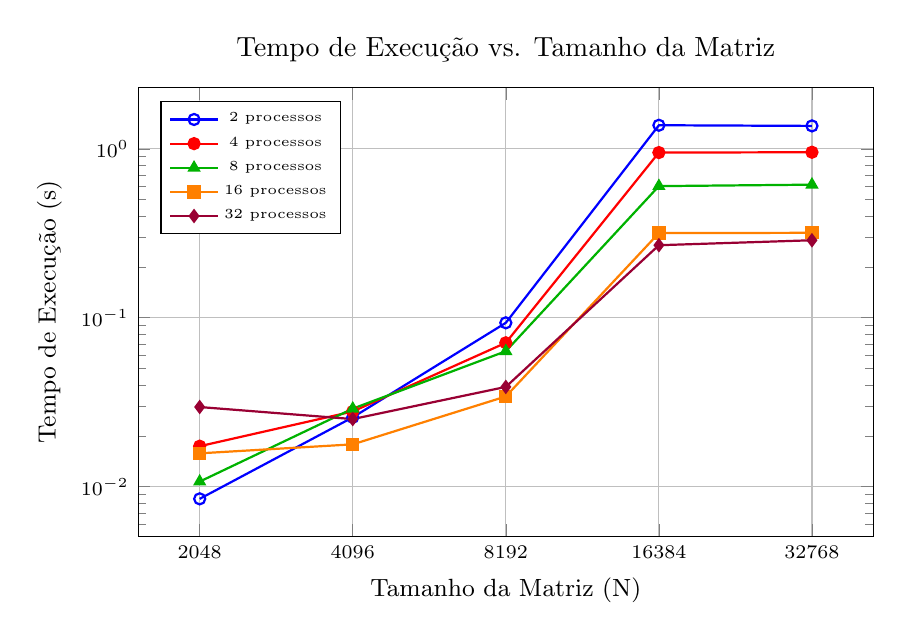
\begin{tikzpicture}
			\begin{axis}[
				title={Tempo de Execu\c{c}\~ao vs. Tamanho da Matriz},
				xlabel={Tamanho da Matriz (N)},
				ylabel={Tempo de Execu\c{c}\~ao (s)},
				xmode=log, % Log scale for matrix size
				ymode=log, % Log scale for time
				legend pos=north west,
				legend style={font=\tiny},
				width=0.9\textwidth,
				height=0.6\textwidth,
				grid=major,
				xtick={2048, 4096, 8192, 16384, 32768},
				xticklabels={2048, 4096, 8192, 16384, 32768},
				ticklabel style={font=\scriptsize},
				label style={font=\small},
				title style={font=\normalsize}
				]
				
				\addplot[color=blue, mark=o, thick]
				coordinates {
					(2048, 0.008465)
					(4096, 0.025716)
					(8192, 0.093287)
					(16384, 1.379384)
					(32768, 1.366954)
				};
				\addlegendentry{2 processos}
				
				\addplot[color=red, mark=*, thick]
				coordinates {
					(2048, 0.017355)
					(4096, 0.027852)
					(8192, 0.071059)
					(16384, 0.950391)
					(32768, 0.954603)
				};
				\addlegendentry{4 processos}
				
				\addplot[color=green!70!black, mark=triangle*, thick]
				coordinates {
					(2048, 0.010708)
					(4096, 0.028952)
					(8192, 0.063350) % Corrected from 0.06335
					(16384, 0.601622)
					(32768, 0.613585)
				};
				\addlegendentry{8 processos}
				
				\addplot[color=orange, mark=square*, thick]
				coordinates {
					(2048, 0.015743)
					(4096, 0.017797)
					(8192, 0.034189)
					(16384, 0.317023)
					(32768, 0.318262)
				};
				\addlegendentry{16 processos}
				
				\addplot[color=purple!80!black, mark=diamond*, thick]
				coordinates {
					(2048, 0.029602)
					(4096, 0.025117)
					(8192, 0.038946)
					(16384, 0.268764)
					(32768, 0.287530) % Corrected from 0.28753
				};
				\addlegendentry{32 processos}
				
			\end{axis}
		\end{tikzpicture}
		\caption{Gráfico de linhas do tempo de execução em função do tamanho da matriz para diferentes números de processos.}
		\label{fig:execution_time_vs_matrix_size}
	\end{figure}
	
	\section{Analise dos Resultados}
	
	\subsection{Variação do Tempo com o Número de Processos}
	
	\hspace{0.62cm}Observa-se que, para matrizes de pequeno porte (por exemplo, 2048 x 2048), o tempo de execução não reduz significativamente com o aumento do número de processos. Na verdade, há uma flutuação: com 2 processos, o tempo foi de aproximadamente 8,4 ms, mas com 4 e 8 processos houve aumento para cerca de 17,3 ms e posterior redução para 10,7 ms, respectivamente.
	
	Esse comportamento se justifica pelo custo de comunicação inerente ao aumento do número de processos, que pode superar os benefícios da paralelização quando o volume de dados por processo é pequeno. Assim, para tamanhos reduzidos de matriz, o overhead de comunicação domina, tornando a execução com mais processos ineficiente.
	
	\subsection{Ganhos de Desempenho com Matrizes Maiores}
	\hspace{0.62cm}À medida que o tamanho da matriz aumenta, o ganho de desempenho com o aumento no número de processos se torna mais evidente:
	
	\begin{itemize}
		\item Para a matriz de 8192 x 8192, o tempo caiu de aproximadamente 93 ms com 2 processos para cerca de 34 ms com 16 processos, e manteve-se baixo com 32 processos.
		
		\item Para a matriz de 16384 x 16384, a redução foi ainda mais expressiva: de 1,37 s com 2 processos para cerca de 0,27 s com 32 processos, mostrando um ganho de quase 5 vezes.
		
		\item O mesmo comportamento foi observado para a maior matriz testada (32768 x 32768), com redução de cerca de 1,36 s para aproximadamente 0,29 s com 32 processos.
	\end{itemize}
	
	Esse comportamento confirma que, para grandes volumes de dados, o custo de comunicação torna-se amortizado pela expressiva redução no tempo de processamento proporcionada pela divisão de trabalho entre múltiplos processos.
	
	\subsection{Análise Comparativa entre Distribuição por Colunas e por Linhas}
	A análise dos resultados revela uma clara dependência entre o tamanho da matriz e a eficiência das duas abordagens de paralelização. Para matrizes pequenas e médias (até 8192x8192), a distribuição por colunas apresenta desempenho competitivo. Isso sugere que, para esses tamanhos, o overhead de comunicação é o fator dominante e a abordagem por colunas consegue um melhor balanceamento da carga computacional. Entretanto, esse cenário se inverte drasticamente quando analisamos matrizes maiores.
	
	Para matrizes grandes (16384x16384 e superiores), a distribuição por linhas demonstra superioridade evidente, sendo 250-370\% mais rápida que a distribuição por colunas. Esta diferença é explicada pela localidade de memória: como C armazena matrizes em formato row-major, o acesso sequencial às linhas aproveita melhor o cache do processador, enquanto o acesso às colunas gera cache misses frequentes que degradam significativamente a performance. Adicionalmente, o overhead dos tipos derivados MPI (\texttt{MPI\_Type\_vector}) necessários para a distribuição por colunas se torna proibitivo conforme o tamanho da matriz aumenta, tornando a abordagem por linhas mais robusta e previsível para aplicações de grande escala.
	
	\section{Conclusão}
	\hspace{0.62cm}A implementação da distribuição por colunas utilizando \texttt{MPI\_Type\_vector} e \texttt{MPI\_Type\_create\_resized} foi realizada com sucesso, permitindo a distribuição de dados não-contíguos e agregação via \texttt{MPI\_Reduce}.
	A análise comparativa revelou que a eficiência é fortemente dependente do tamanho da matriz. Para matrizes menores a distribuição por colunas foi competitiva, mas para matrizes grandes (16384x16384) tornou-se 250-370\% mais lenta devido aos cache misses causados pelo acesso não-sequencial em formato row-major do C. O overhead dos tipos derivados MPI também se intensifica com o tamanho da matriz, tornando a distribuição por linhas mais adequada para aplicações de grande escala.
	
\end{document}
